\chapter{LAB Session 01 -- CMOS Current Mirror Design and Analysis}

\subsection*{MOSFET PARAMETERS FOR HAND CALCULATION}

\begin{center}
\resizebox{\textwidth}{!}{
\begin{tabular}{|c|c|c|c|c|c|c|}
\hline
 & $k'_{n/p}$ [$\mu$A/V$^2$] & $\eta$ [V/m] & $\chi = \frac{g_{mb}}{g_m}$ & $C_{ox}$ [fF/$\mu$m$^2$] & $C_{GS0}=C_{GD0}$ [fF/$\mu$m] & $C_{jd/s}$ [fF/$\mu$m] (*) \\
\hline
nMOSFET & 470 & $1.1 \cdot 10^7$ & 0.2 & 11.2 & 0.32 & 0.45 \\
\hline
pMOSFET & 100 & $1.5 \cdot 10^7$ & 0.2 & 11.2 & 0.32 & 0.70 \\
\hline
\end{tabular}
}
\end{center}
\vspace{0.4cm}
\subsection*{PROCESS VARIATION AND DEVICE MISMATCH PARAMETERS FOR HAND CALCULATION}

\begin{center}
\begin{tabular}{|c|c|c|c|c|}
\hline
 & $V_{TN/P}$ [V] & $k'_{n/p}$ [mA/V$^2$] & $A_{\Delta VT}$ [mV$\cdot\mu$m] & $A_{Dk/k}$ [\%\,$\cdot\mu$m] \\
\hline
nMOSFET & 
\begin{tabular}{c}
0.31 (min) \\
0.37 (typ) \\
0.44 (max)
\end{tabular}
&
\begin{tabular}{c}
376 (min) \\
470 (typ) \\
564 (max)
\end{tabular}
& 5 & 1.1 \\
\hline
pMOSFET & 
\begin{tabular}{c}
-0.26 (min) \\
-0.33 (typ) \\
-0.40 (max)
\end{tabular}
&
\begin{tabular}{c}
80 (min) \\
100 (typ) \\
120 (max)
\end{tabular}
& 3.6 & 1 \\
\hline
\end{tabular}
\end{center}

\section{Schematic and Testbench Configuration}

% Inserire schematico
\begin{figure}[H]
    \centering
    \begin{minipage}{0.48\linewidth}
        \centering
        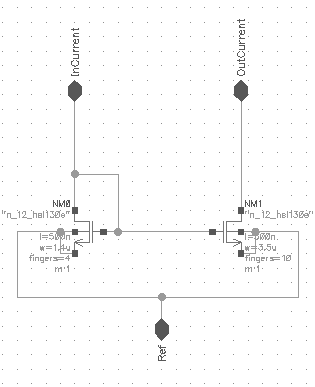
\includegraphics[width=\linewidth]{images/n_type_schematics_L500nm (1).png}
    \end{minipage}
    \hfill
    \begin{minipage}{0.48\linewidth}
        \centering
        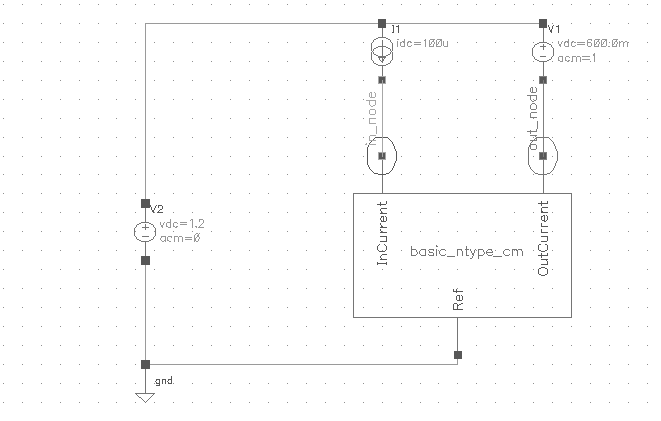
\includegraphics[width=\linewidth]{images/nmos_tb.png}
    \end{minipage}
    \caption{nMOS schematic and testbench}
\end{figure}
\section{DC and Small-Signal Characterization of the Basic Mirror}

\subsection{Output Current Behaviour Under DC Sweep}

A DC sweep of the output voltage $V1$ from 0 V to 1.2 V has been performed. The output current $I_{OUT}$ has been plotted together with the ideal mirrored current $N \cdot I_{IN}$.

\begin{figure}[H]
    \centering
    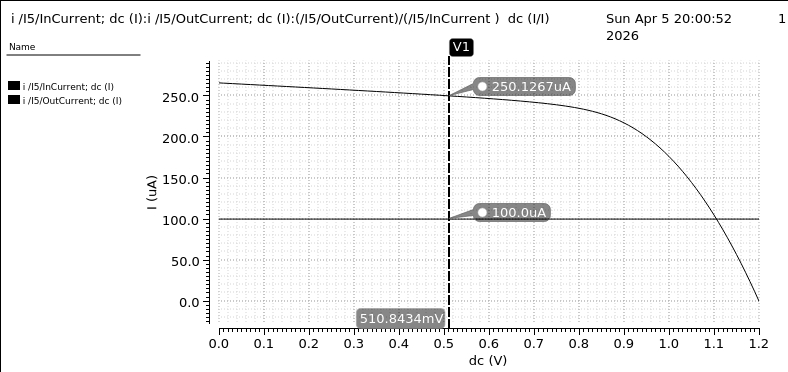
\includegraphics[width=1.0\linewidth]{images/i_o_V_i_in.jpg}
    \caption{$I_{OUT}$ vs $V_1$ with $N \cdot I_{IN}$ reference}
\end{figure}

The results show that $I_{OUT}$ initially decreases slowly and almost linearly as $V_1$ increases due to channel length modulation (CLM).
As $V_1$ increases further, the current exhibits a steeper and nonlinear decrease. In this region, the output transistor progressively leaves the saturation region and enters the triode region, leading to a more pronounced reduction of the drain current and a significant deviation from the ideal current-mirror behavior.

% Correction: Changed \begin{equation*} to \begin{equation} to match the \label and subsequent reference (\ref{eq:current_error}).
A marker has been placed at the point where $I_{OUT} = N \cdot I_{IN}$. At this point:
\begin{itemize}
    \item $V_1 = 510.84\,\text{mV}$
\end{itemize}
The equality holds only at this specific value of $V_1$ due to CLM and the originated current error can be approximated as:
\begin{equation}
\Delta I_o \approx \frac{V_{DS1} - V_{DS2}}{R_o}
\label{eq:current_error}
\end{equation}

It can be observed from (\ref{eq:current_error}) that the current error depends on the difference between $V_{DS1}$ and $V_{DS2}$. Since $V_{DS1}$ is fixed by the reference branch, while $V_{DS2}$ varies with the swept output voltage $V_1$, the condition $V_{DS1} = V_{DS2}$ is satisfied only at a single value of $V_1$. 
\subsection{Low-Frequency Output Resistance from AC Response}

An AC analysis has been carried out by applying a small-signal voltage source at the current-mirror output node, with AC magnitude equal to 1 V, around the selected DC operating point. Therefore, the magnitude and phase of the output current are respectively the magnitude and phase of the output admittance.

\begin{figure}[H]
    \centering
    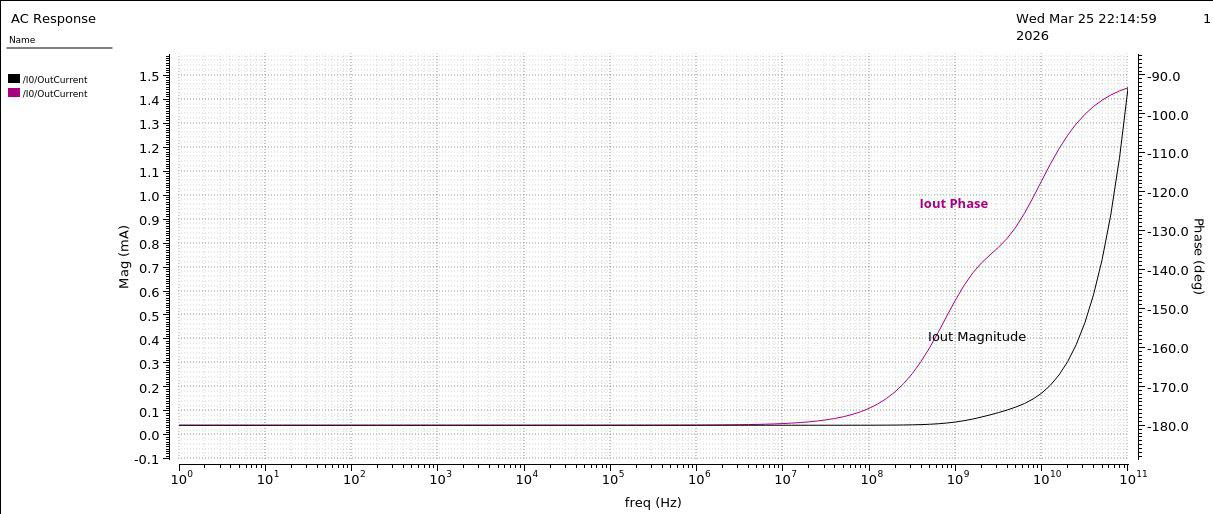
\includegraphics[width=0.8\linewidth]{images/AC phase.jpeg}
    \caption{Magnitude and phase of the output current, corresponding to the output admittance}
\end{figure}

The low-frequency value of the admittance magnitude has been extracted from the AC plot as:

\begin{equation*}
|Y_{out}(0)| \approx 39.92 \,\mu S
\end{equation*}
\begin{figure}[H]
    \centering
    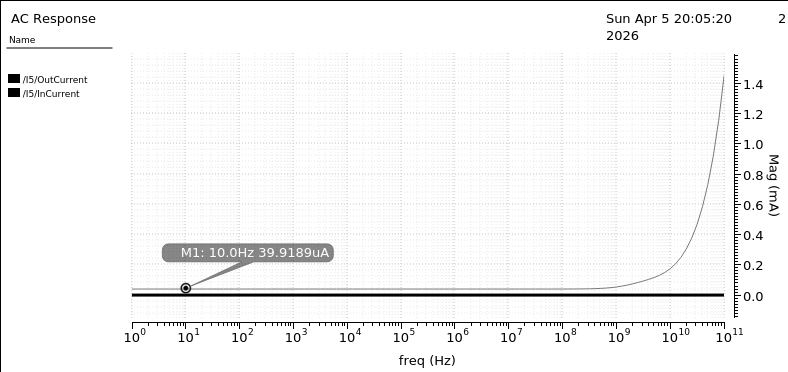
\includegraphics[width=0.8\linewidth]{imagesV2/AC_analysis_marked.jpg}
    \caption{Low-frequency value of the admittance magnitude}
\end{figure}
The corresponding output resistance is then estimated as:

\begin{equation*}
R_o = \frac{1}{|Y_{out}(0)|} \approx 25.05 \, k\Omega
\end{equation*}
This value must be compared with the output admittance obtained from the DC sweep. In particular, the small-signal admittance at DC is given by the local slope of the $I_{OUT}$--$V_1$ characteristic, evaluated at the same operating point used for the AC simulation:
\begin{equation*}
Y_{out}(0)=\left.\frac{dI_{OUT}}{dV_1}\right|_{Q=510.84mV}=34.82\mu S
\end{equation*}
The relative error between the two estimations is:

\begin{equation*}
\text{Error} = \frac{|Y_{out}^{AC} - Y_{out}^{DC}|}{Y_{out}^{AC}} \approx 12.8\%
\end{equation*}
The discrepancy between the AC and DC result is primarily 
attributed to the mismatch in the operating point ($Q$-point). In the AC 
calculations, the operating point was constrained by the fixed DC voltage 
connected to the output node, where $V_{DC} = 600 \, \text{mV}$. 

Conversely, the precise operating point of the MOSFET was determined to be 
$510.84 \, \text{mV}$, corresponding to the condition $I_o = 2.5 I_{in}$. 
Although quantization steps in the simulation prevented the evaluation of the 
exact point where the current ratio perfectly matches the ideal value, this 
quantization error is negligible. The primary source of divergence is the 
offset between the software's operating point and the analytical operating 
point used in the admittance derivation.
\subsection{Output impedance frequency behaviour}
According to the small-signal equivalent circuit, the output impedance can be modeled as:

\begin{equation*}
Z_{out}(s)=\frac{r_{o2}}{1+s r_{o2}[C_{db2}+(N+1)C_{gd2}]}
\end{equation*}
Where the intersted parasitic capacitances are evaluated from process parameters as:

\begin{equation*}
C_{gd2} = C_{gd0}\cdot W = 0.32\,\frac{\text{fF}}{\mu m} \cdot 3.5\,\mu m = 1.12\,\text{fF}
\end{equation*}

\begin{equation*}
C_{db2} = C_{jn}\cdot W = 0.45\,\frac{\text{fF}}{\mu m} \cdot 3.5\,\mu m =1.58\,\text{fF}
\end{equation*}

The dominant pole of the output impedance is therefore:
\begin{equation*}
f_p = \frac{1}{2\pi r_{o2}\left[C_{db2}+(N+1)C_{gd2}\right]} \approx 1.318\,\text{GHz}
\end{equation*}
\begin{figure}[H]
    \centering
    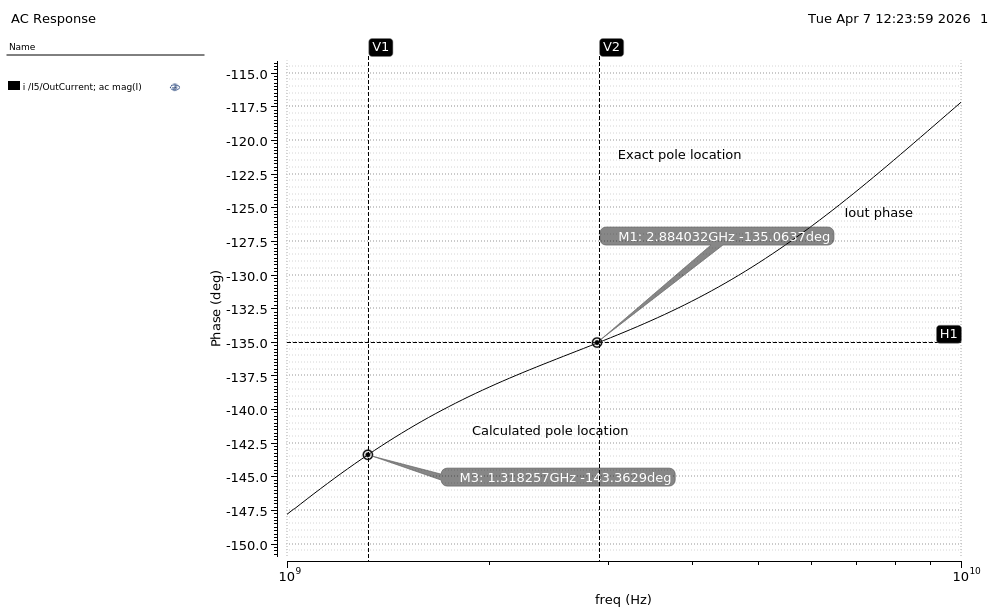
\includegraphics[width=1.0\linewidth]{imagesV2/phase_mag_annot_exact.png}
    \caption{Phase response of the output admittance. Markers highlight the theoretical pole}
\end{figure}
The theoretical behavior of the output impedance is confirmed by the simulation results. At low frequency, the output impedance is purely resistive and approximately equal to $r_{o2}$, corresponding to the flat region observed in the AC response.
The phase response is also consistent with the theoretical model. In particular, a phase shift is observed around the pole frequency, marking the transition from resistive to capacitive behavior.
From the phase plot, the actual pole frequency can be identified as the point where the phase reaches approximately $-135^\circ$. From the simulation results, this occurs at:
\begin{equation*}
f_{p,real} = 2.88\,\text{GHz}
\end{equation*}
The discrepancy between the theoretical and simulated pole frequencies is mainly due to parasitic capacitances and higher-order effects, which are not fully captured by the simplified analytical model.
\subsection{DC Analysis with Gate Length and Finger Width Variations}
First, the effect of the gate length has been investigated. The minimum and maximum values have been set to $L_{min} = 100\,\text{nm}$ and $L_{max} = 500\,\text{nm}$, respectively. The simulator automatically selected 10 intermediate points within this range, allowing to highlight the dependence of the output current on the transistor channel length.

\begin{figure}[H]
    \centering
    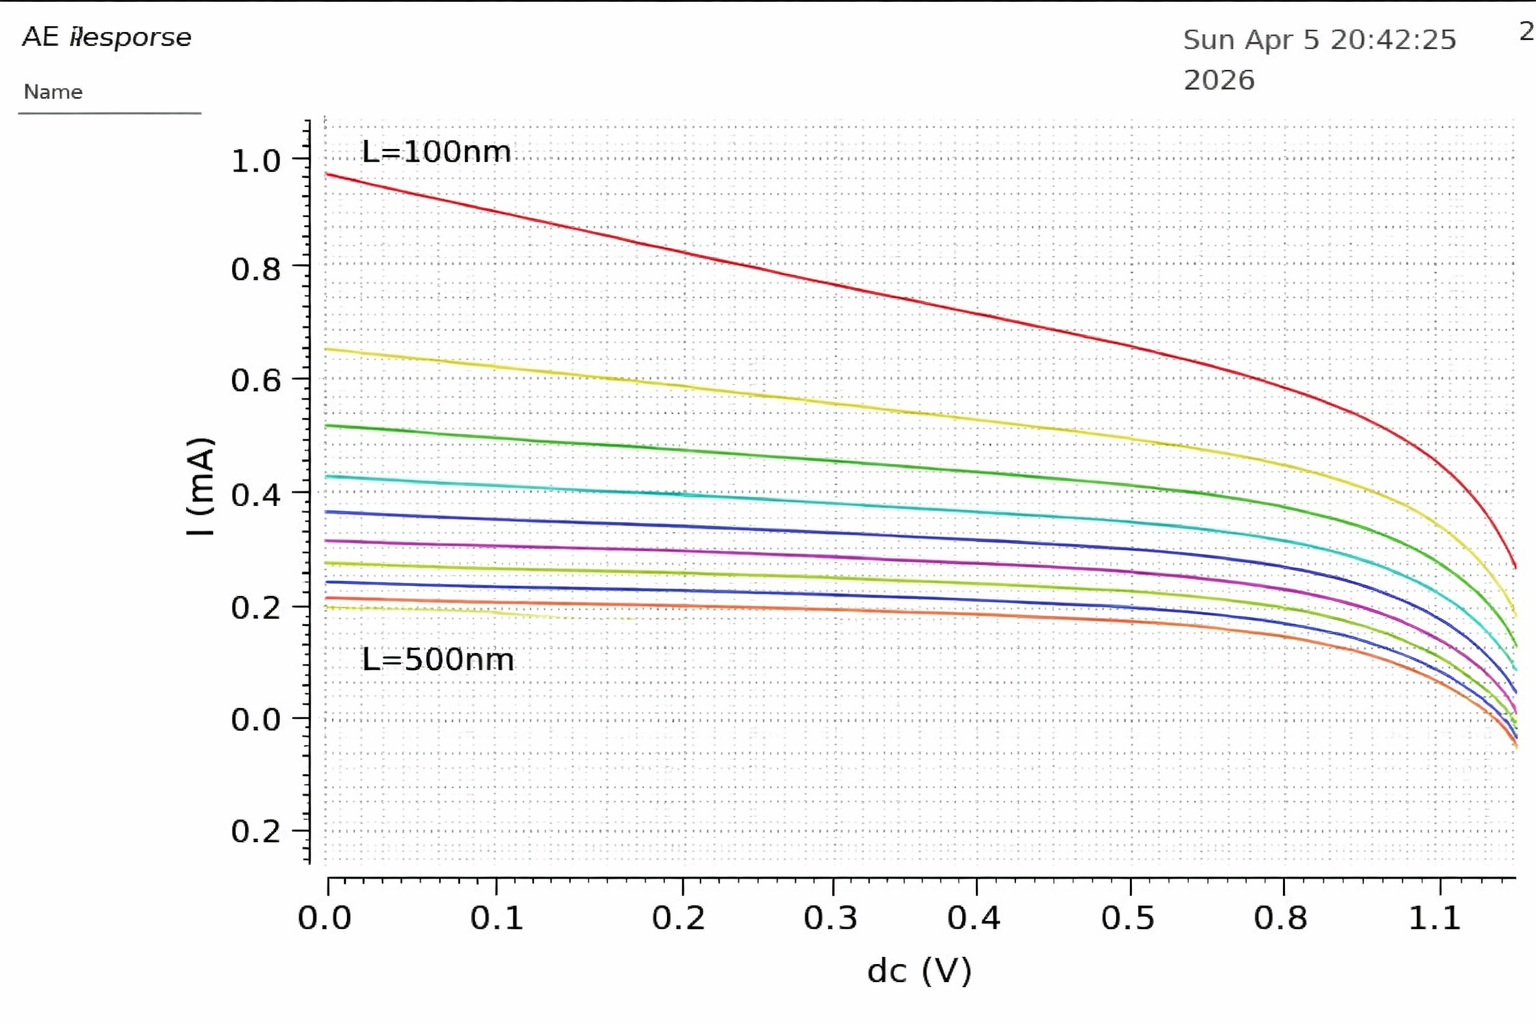
\includegraphics[width=0.82\linewidth]{images/Curva di corrente per lunghezze canale.png}
    \caption{DC output current $I_{OUT}$ as a function of the output voltage for different values of the gate length $L$, ranging from $100\,\text{nm}$ to $500\,\text{nm}$. The curves show how the transistor length affects the output current.}
    \label{fig:cm_dc_variants}
\end{figure}

\begin{figure}[H]
    \centering
    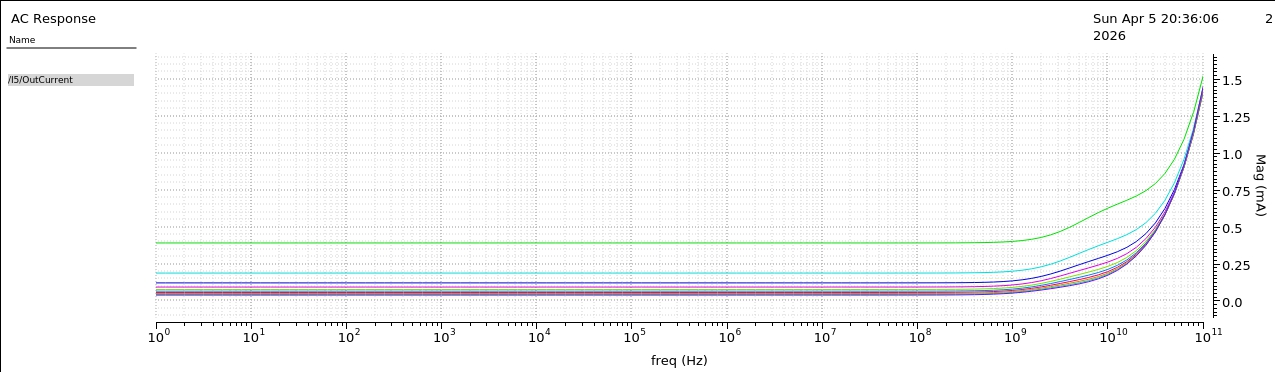
\includegraphics[width=1.00\linewidth]{imagesV2/I_o_ac_DiffrentL.jpg}
    \caption{AC response of the current mirror for different gate lengths $L$.}
    \label{fig:cm_ac_variants}
\end{figure}

In a second step, the effect of transistor layout has been analyzed by varying the number of fingers of transistor $M_2$. In particular, two configurations have been considered: 4 fingers and 10 fingers, keeping the total width and length consistent with the original design.

\begin{figure}[H]
    \centering
    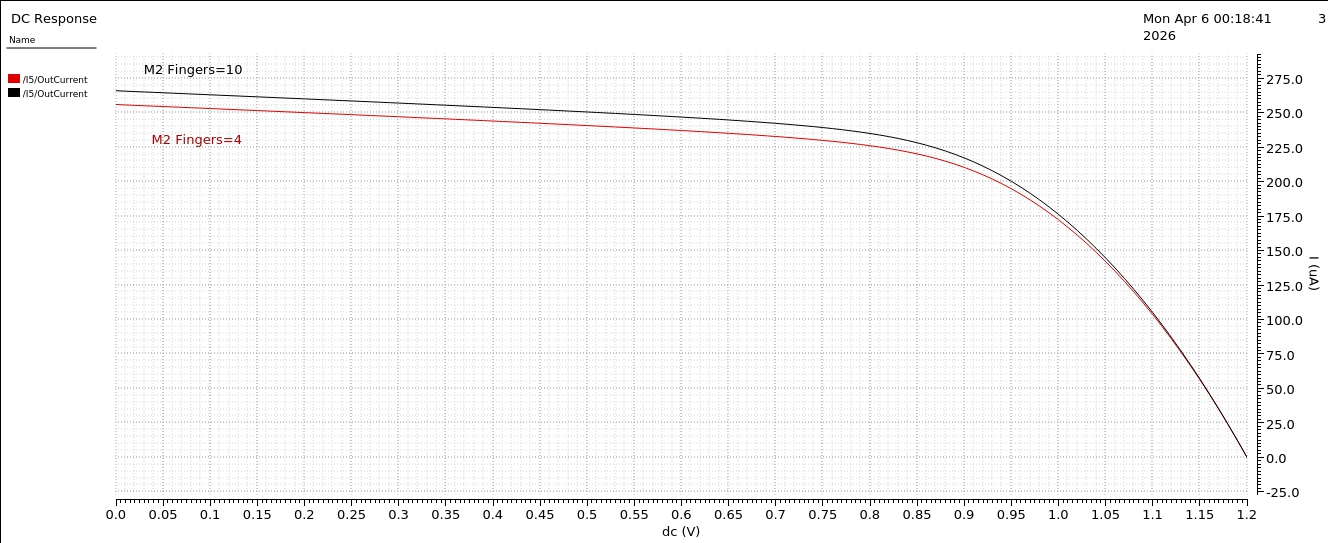
\includegraphics[width=0.82\linewidth]{imagesV2/DC4-10.jpg}
    \caption{DC output characteristics of the current mirror for two different finger configurations of $M_2$ (4 and 10 fingers).}
    \label{fig:4_10dc_variants}
\end{figure}

\begin{figure}[H]
    \centering
    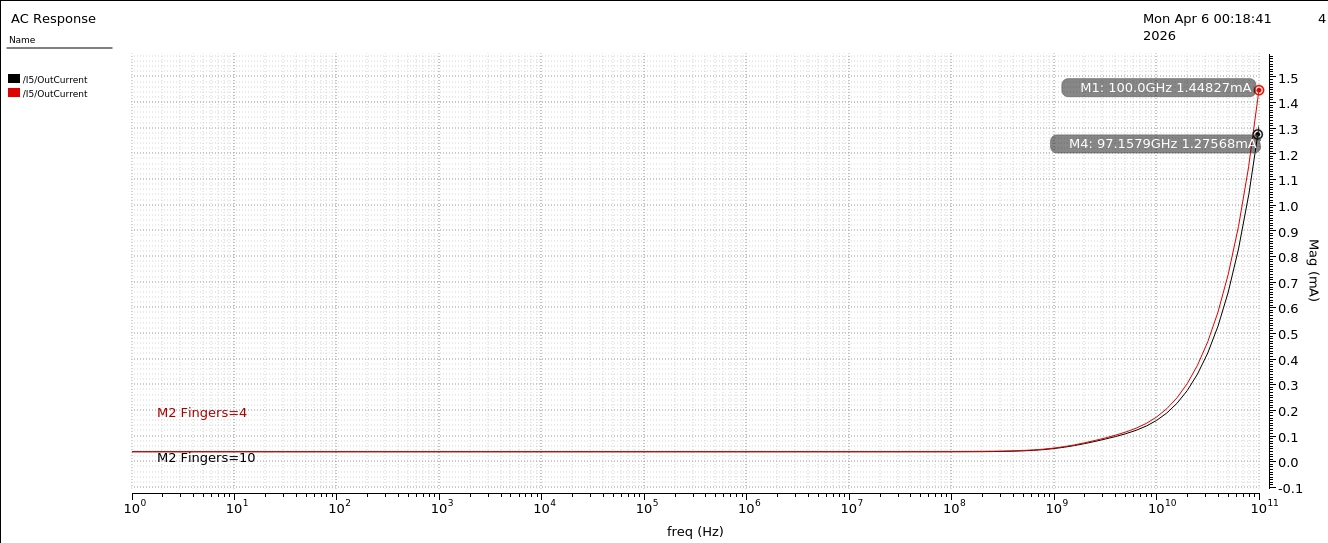
\includegraphics[width=0.82\linewidth]{imagesV2/AC4-10.jpg}
    \caption{AC response of the current mirror for different finger configurations of $M_2$ (4 and 10 fingers).}
    \label{fig:4_10ac_variants}
\end{figure}
\subsubsection{Discussion of Results}
\paragraph{Effect of $L_1\neq L_2$:}
It is important to distinguish the role of the two transistors in this analysis. For $M_1$, the reference current $I_{REF}$ is externally imposed and fixed to $100\,\mu\text{A}$. In contrast, for $M_2$ the drain current is not imposed, but results from the mirror action and from the actual device geometry. Therefore, when the channel length of $M_2$ is reduced, the output current $I_O$ increases, and this is consistent with the MOS saturation-current expression:
\begin{equation*}
I_D \approx \frac{1}{2}\mu C_{ox}\frac{W}{L}(V_{GS}-V_{th})^2(1+\lambda V_{DS}),
\end{equation*}
because a shorter channel directly increases the factor $W/L$. In addition, in the considered range the threshold voltage of $M_2$ also changes with $L$, but the sweep shows that the dominant effect on the current is the explicit dependence on $1/L$ in the previous equation. As a result, shorter values of $L_2$ produce larger values of $I_O$.

%\begin{figure}[H]
 %   \centering
  %  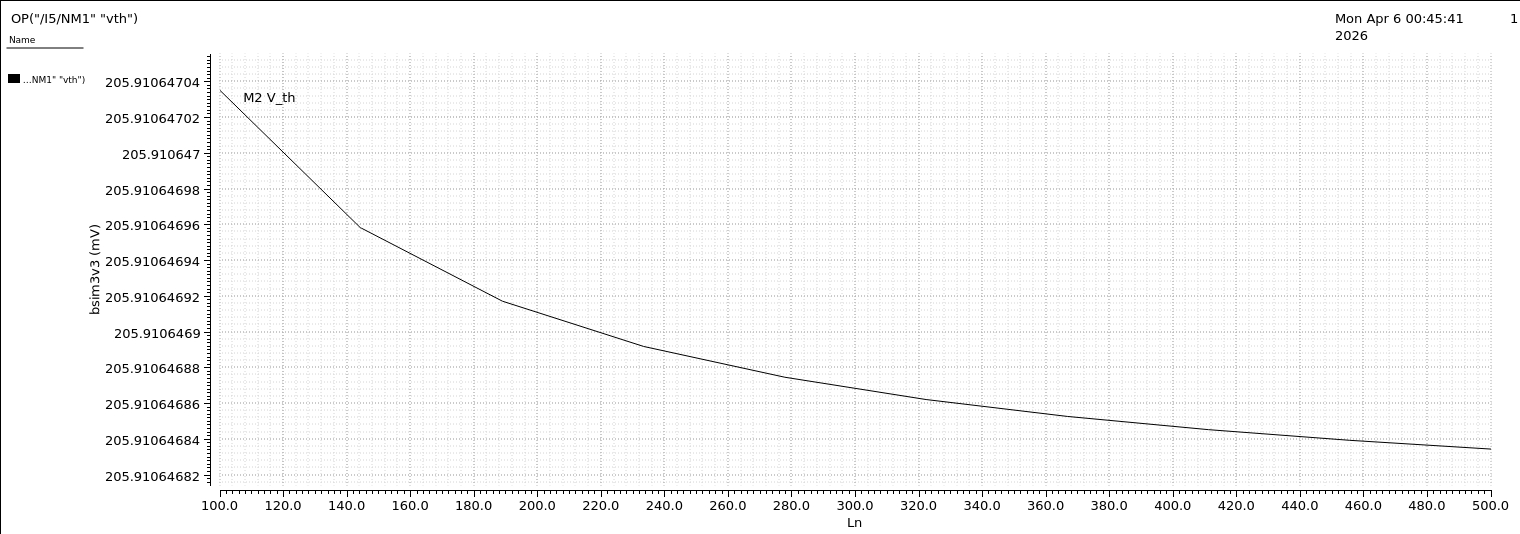
\includegraphics[width=0.8\linewidth]{images/Vth_L.jpg}
   % \caption{Sweep of the channel length of $M_2$ and corresponding variation of its threshold voltage $V_{th,2}$.}
    %\label{fig:M2_L_Vth_sweep}
%\end{figure}
\paragraph{Effect of different number of fingers for M2:}
A similar interpretation applies to the case with a different number of fingers. According to the qualitative plot of $V_T$ versus $W$ at fixed $L$, the threshold voltage also depends (although more weakly) on the effective device width. Changing the number of fingers modifies how the total width is physically distributed, thus altering the effective geometry of the transistor and introducing layout-dependent effects. In the considered case (Number of Fingers = 4 for $M_2$), the output current curve deviates from the nominal one even though the overall $W$ and $L$ are kept consistent with the original design. This is because the different finger configuration changes the effective threshold voltage and the parasitic elements of the device. As a result, the current mirror no longer perfectly replicates the reference current, and a visible deviation appears along the entire sweep. Compared to the channel length variation, this effect is generally smaller, but still significant, confirming that both device geometry and layout implementation impact the accuracy of the current mirror.



\section{Assessment of process spread and device mismatch }
Process corner simulations have been performed for the following conditions: Typical (TYP, 27°C), Slow-Slow (SS, -20°C), and Fast-Fast (FF, 85°C).

\subsection{Process Corner Evaluation}

\begin{table}[h!]
\centering
\caption{Current Mirror Performance Across Process Corners}
\label{table:corners_corrected}
\begin{tabular}{|l|c|c|}
\hline
\textbf{Corner} & \textbf{$V_{IN}$ [mV]} & \textbf{$\Delta I_{OUT}$ [$\mu$A]} \\ \hline
TYP (27 °C)     & 686.0                  & -3.096                             \\ \hline
SS (-20 °C)     & 751.4                  & -5.516                             \\ \hline
FF (85 °C)      & 630.8                  & -1.155                             \\ \hline
\end{tabular}
\end{table}




The variations observed in $V_{IN}$ and $\Delta I_{OUT}$ across the simulated process corners (\textbf{TYP}, \textbf{SS}, and \textbf{FF}) are primarily driven by the global fluctuations in the threshold voltage ($V_{th}$) and carrier mobility ($\mu$). These dependencies are governed by the MOSFET saturation current equation:

\begin{equation*}
I_D \approx \frac{1}{2} \mu C_{ox} \frac{W}{L} (V_{GS} - V_{th})^2 (1 + \lambda V_{DS})
\end{equation*}
\subsubsection{Discussion of Results}
\paragraph{Input Voltage ($V_{IN}$) Sensitivity}:
In the \textbf{SS (Slow-Slow)} corner at \textbf{$-20$°C}, the devices show the highest threshold voltage and degraded mobility. To hold the fixed reference current of $100\,\mu$A, the gate-source voltage ($V_{GS} = V_{IN}$) must increase to compensate for the "weak" drive capability. This resulted in the observed maximum $V_{IN}$ of \textbf{751.4\,mV}. 

Conversely, in the \textbf{FF (Fast-Fast)} corner at \textbf{85°C}, the significant reduction in $V_{th}$ dominates the temperature-induced mobility decrease. Consequently, the transistors reach the target current with a lower overdrive voltage, leading to a minimum $V_{IN}$ of \textbf{630.8\,mV}. The total spread of \textbf{120.6\,mV} represents the impact of global process and temperature variation on the biasing point.



\paragraph{Output Current Error ($\Delta I_{OUT}$)}:

For an n-type current mirror, the relationship between the reference current ($I_{REF}$) and the output current ($I_{OUT}$) is defined by the aspect ratios and the channel length modulation effect:

\begin{equation*}
I_{OUT} = N \cdot I_{REF} \cdot \frac{1 + \lambda V_{DS2}}{1 + \lambda V_{DS1}}
\end{equation*}

where $N = 2.5$ and $I_{REF} = 100\,\mu$A, yielding an ideal $I_{OUT}$ of $250\,\mu$A. The current error is defined as $\Delta I_{OUT} = I_{OUT} - 250\,\mu$A. The simulation results show:

\begin{itemize}
    \item \textbf{Negative Error Trend:} The error remains negative across all corners, indicating $I_{OUT} < 250\,\mu$A. This suggests that $V_{DS1} > V_{DS2}$ in the DC operating point, or that the effective $\lambda$ at these lengths reduces the output current more than predicted.
    
    \item \textbf{SS Corner ($-5.516\,\mu$A):} At $-20$°C, the transistors exhibit lower channel length modulation ($\lambda$) but higher $V_{th}$ mismatch sensitivity. The larger error magnitude suggests a significant discrepancy between the drain-source voltages of the mirror pair at this cold temperature.
    
    \item \textbf{FF Corner ($-1.155\,\mu$A):} The error is minimized under "fast" conditions at $85$°C. This is due to the higher transconductance ($g_m = \mu C_{ox} \frac{W}{L}(V_{GS}-V_{th})$) of the devices, which makes the output current more robust against small voltage offsets between the input and output nodes.
\end{itemize}
\subsection{Monte Carlo Analysis of Current and Input-Voltage Spread}

A Monte Carlo simulation ($N=100$) was performed to evaluate the impact of local device mismatch and global process variations on the current mirror's performance. The extracted mean values ($\mu$) and standard deviations ($\sigma$) from these distributions are summarized in Table \ref{table:monte_carlo}.

\begin{figure}[H]
    \centering
    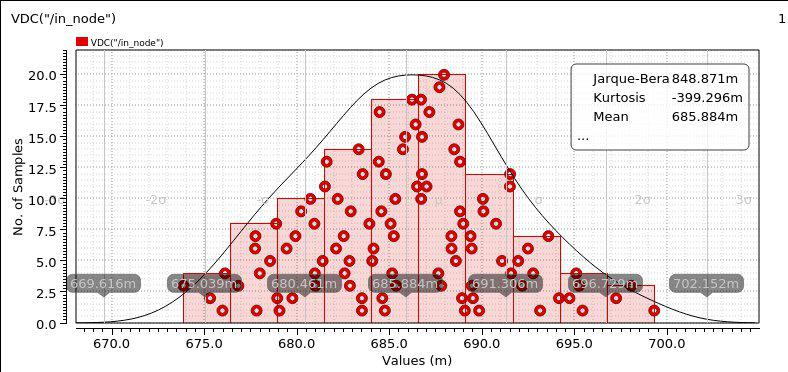
\includegraphics[width=0.8\linewidth]{images/vcd_montecarlo.JPG}
    \caption{Monte Carlo distribution of $V_{IN}$.}
    \label{fig:vcd_montecarlo}
\end{figure}

\begin{figure}[H]
    \centering
    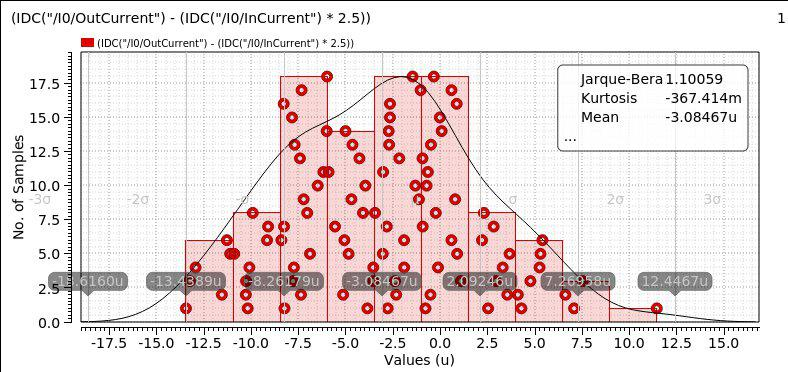
\includegraphics[width=0.8\linewidth]{images/currents_montecarlo.JPG}
    \caption{Monte Carlo distribution of $\Delta I_{OUT}$.}
    \label{fig:currents_montecarlo}
\end{figure}

\begin{table}[h!]
\centering
\caption{Monte Carlo Statistical Results ($N=100$)}
\label{table:monte_carlo}
\begin{tabular}{|l|c|c|}
\hline
\textbf{Variable} & \textbf{Mean} & \textbf{Std. Deviation ($\sigma$)} \\ \hline
Input Voltage $V_{IN}$ [mV]     & 685.88                & 5.42                               \\ \hline
Current Error $\Delta I_{OUT}$ [$\mu$A] & -3.085                   & 5.18                               \\ \hline
\end{tabular}
\label{Fig:table_montecarlo}
\end{table}
\paragraph{Systematic vs. Random Error}
As observed in the histograms, the mean value of the current error $\Delta I_{OUT}$ is $-3.085\,\mu$A rather than zero. This represents the \textbf{systematic error} of the design, primarily caused by the $V_{DS}$ mismatch between the input and output branches of the simple current mirror. The standard deviation $\sigma = 5.18\,\mu$A represents the random mismatch inherent in the manufacturing process.

\paragraph{Mismatch Verification}
To verify the consistency of the simulation, the Pelgrom mismatch model is applied using the parameters $A_{\Delta VT} = 5\,\text{mV}\cdot\mu\text{m}$ and $A_{Dk/k} = 1.1\,\%\cdot\mu\text{m}$. For a device area $W \cdot L = 1.75\,\mu\text{m}^2$:

\begin{equation*}
\sigma_{\Delta VT} = \frac{A_{\Delta VT}}{\sqrt{W \cdot L}} = 3.78\,\text{mV}, \quad \sigma_{\Delta k/k} = \frac{A_{Dk/k}}{\sqrt{W \cdot L}} = 0.0083
\end{equation*}

The total relative current mismatch is estimated as:
\begin{equation*}
\sigma_{\Delta I/I} = \sqrt{\sigma_{\Delta k/k}^2 + \left( \frac{2}{V_{GS} - V_{th}} \sigma_{\Delta VT} \right)^2} \approx 2.53\%
\end{equation*}

For an ideal $I_{OUT} = 250\,\mu$A, the calculated standard deviation is:
\begin{equation*}
\sigma_{calc} = 250\,\mu\text{A} \cdot 0.0253 = 6.32\,\mu\text{A}
\end{equation*}

\paragraph{Comparison of Statistical and Deterministic Distributions}

A critical comparison is made between the global process corners and the local statistical variations. For the input bias voltage $V_{IN}$, the Monte Carlo simulation yielded a standard deviation $\sigma_{V_{IN}} = 5.42\,\text{mV}$. The $3\sigma$ confidence interval, which covers $99.7\%$ of the statistical samples, is calculated as:
\begin{equation*}
\Delta V_{IN, 3\sigma} = 6 \cdot \sigma_{V_{IN}} = 6 \cdot 5.42\,\text{mV} \approx 32.52\,\text{mV}
\end{equation*}

In contrast, the deterministic corner analysis (from SS at $-20^\circ$C to FF at $85^\circ$C) showed a spread of:
\begin{equation*}
\Delta V_{IN, corners} = V_{IN,SS} - V_{IN,FF} = 751.4\,\text{mV} - 630.8\,\text{mV} = 120.6\,\text{mV}
\end{equation*}
Regarding the output current accuracy, the simulated standard deviation of the error $\sigma_{\Delta I, sim} = 5.18\,\mu$A was compared to the Pelgrom calculation derived earlier:
\begin{equation*}
\sigma_{\Delta I, calc} = I_{OUT, ideal} \cdot \sqrt{\frac{A_{Dk/k}^2}{WL} + \left( \frac{2}{V_{OV}} \frac{A_{\Delta VT}}{\sqrt{WL}} \right)^2} \approx 6.32\,\mu\text{A}
\end{equation*}

\section{Wide-Swing Cascode Current Mirror (WS-CCM)}

\subsection{Schematic and Testbench Configuration}

The wide-swing cascode current mirror (WS-CCM) has been implemented according to the design specifications. The circuit schematic and the corresponding testbench are shown in Fig.~\ref{fig:cascode_schematic_tb}.

\begin{figure}[H]
    \centering
    \begin{minipage}{0.46\linewidth}
        \centering
        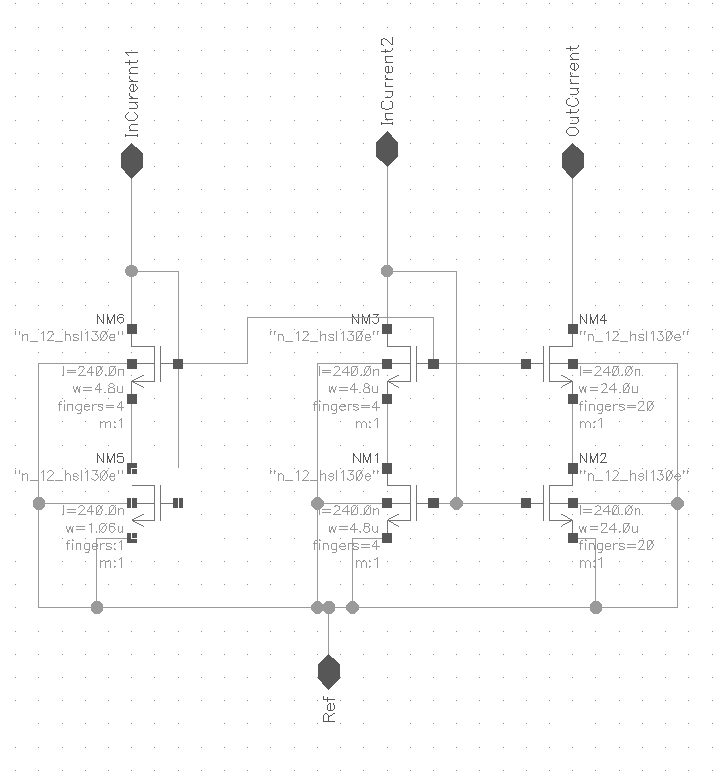
\includegraphics[width=\linewidth]{imagesV2/schematics_w_1.06.png}
    \end{minipage}
    \hfill
    \begin{minipage}{0.46\linewidth}
        \centering
        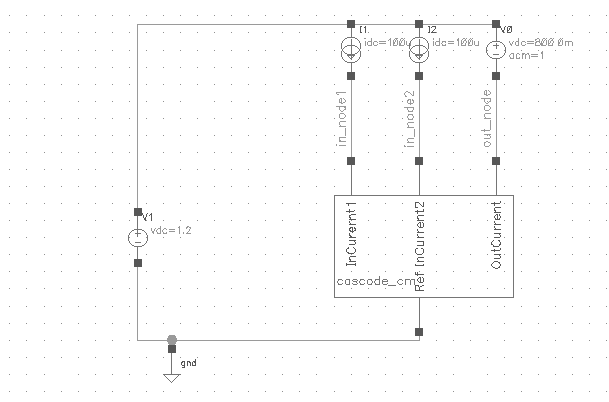
\includegraphics[width=\linewidth]{imagesV2/tb_cascode_schematics (1).png}
    \end{minipage}
    \caption{WS-CCM schematic (left) and testbench (right)}
    \label{fig:cascode_schematic_tb}
\end{figure}

\subsection{Operating Point Adjustment}

A parametric sweep of the transistor $M_5$ width has been performed in order to properly bias the circuit. The final value has been selected as the point at which the family of curves corresponding to $V_{DS1}$, $V_{DS2}$, $V_{DS3}$ and $V_{DS4}$ is overall closest to the target value of $0.25\,\text{V}$.

The final selected value is:

\begin{equation*}
W_{M5} = 1.06\,\mu\text{m}, \quad L_{M5} = 240\,n\text{m}
\end{equation*}
\begin{figure}[H]
    \centering
    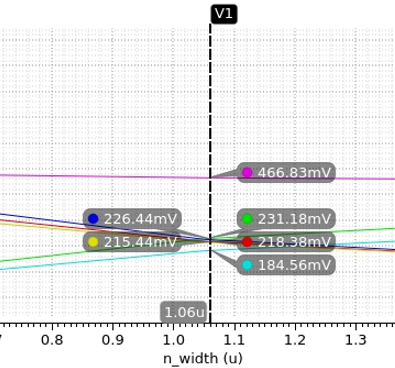
\includegraphics[width=0.5\linewidth]{imagesV2/Screenshot 2026-04-04 100809.png}
    \caption{Family of curves of $V_{DS1}$, $V_{DS2}$, $V_{DS3}$ and $V_{DS4}$ as a function of $W_5$.}
    \label{fig:vds_sweep}
\end{figure}

\begin{figure}[H]
    \centering
    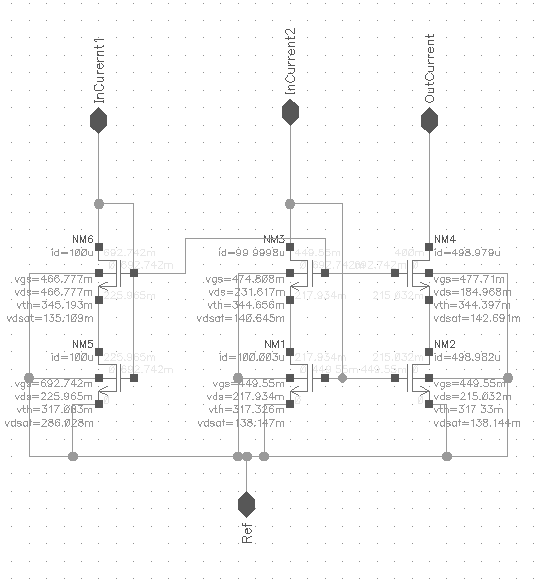
\includegraphics[width=0.65\textwidth]{chapters/M5_op.png} 
    \caption{Cascode schematics with operating points and node voltages.}
    \label{fig:cascode_op}
\end{figure}

The resulting operating point values for the cascode current mirror are summarized in Table 1.3:

\begin{table}[H]
    \centering
    \caption{Measured DC Operating Point Parameters}
    \label{table:operating_points}
    \begin{tabular}{lc}
        \toprule
        \textbf{Parameter} & \textbf{Value [mV]} \\
        \midrule
        $V_{DS1}$          & 226.44              \\
        $V_{DS2}$          & 215.40              \\
        $V_{DS3}$          & 231.20              \\
        $V_{DS4}$          & 184.60              \\
        $V_{G6}$           & 692.74              \\
        \bottomrule
    \end{tabular}
\end{table}
The selection of the optimal value of $W_5$ is driven by a design trade-off. In principle, it would have been possible to choose a point where $V_{DS1}$ and $V_{DS2}$ are exactly equal to $250\,\text{mV}$. However, in that case, $V_{DS3}$ and $V_{DS4}$ would have deviated significantly from the target value of $250\,\text{mV}$. Therefore, a compromise solution has been adopted, selecting the value of $W_5$ for which all four drain-source voltages are as close as possible to the desired target simultaneously.

\subsection{DC Sweep Analysis}

A DC sweep of the output voltage $V_{OUT}$ has been performed. The resulting output current $I_{OUT}$ has been compared with the ideal mirrored current:

\begin{figure}[H]
    \centering
    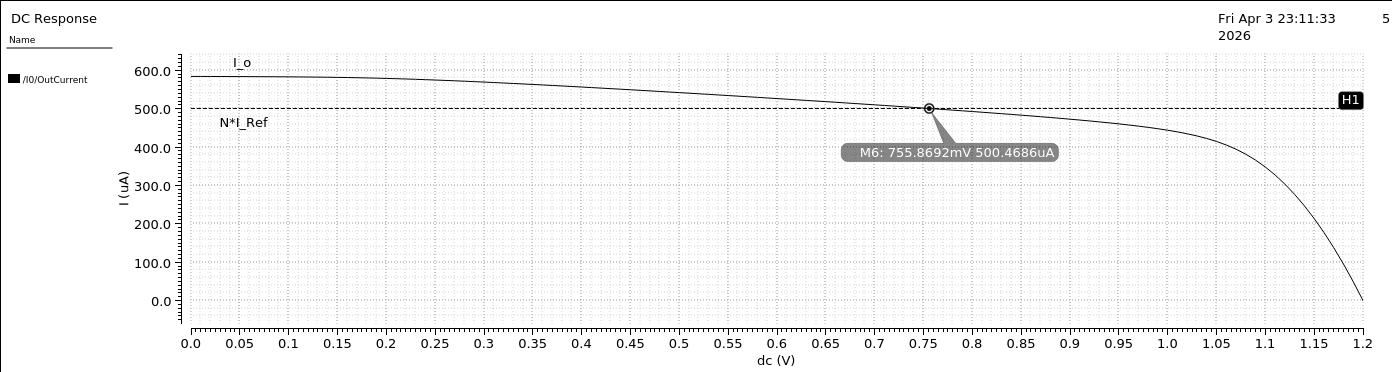
\includegraphics[width=1.00\linewidth]{imagesV2/I_o_vs_I_ref.jpg}
    \caption{DC sweep: $I_{OUT}$ and ideal current comparison with marker}
\end{figure}

\subsection{AC Analysis and Output Resistance}

An AC analysis has been carried out by applying a small-signal excitation of 1 V at the output node. Under this condition, the output current corresponds to the output admittance as it happened for the CM:

\begin{figure}[H]
    \centering
    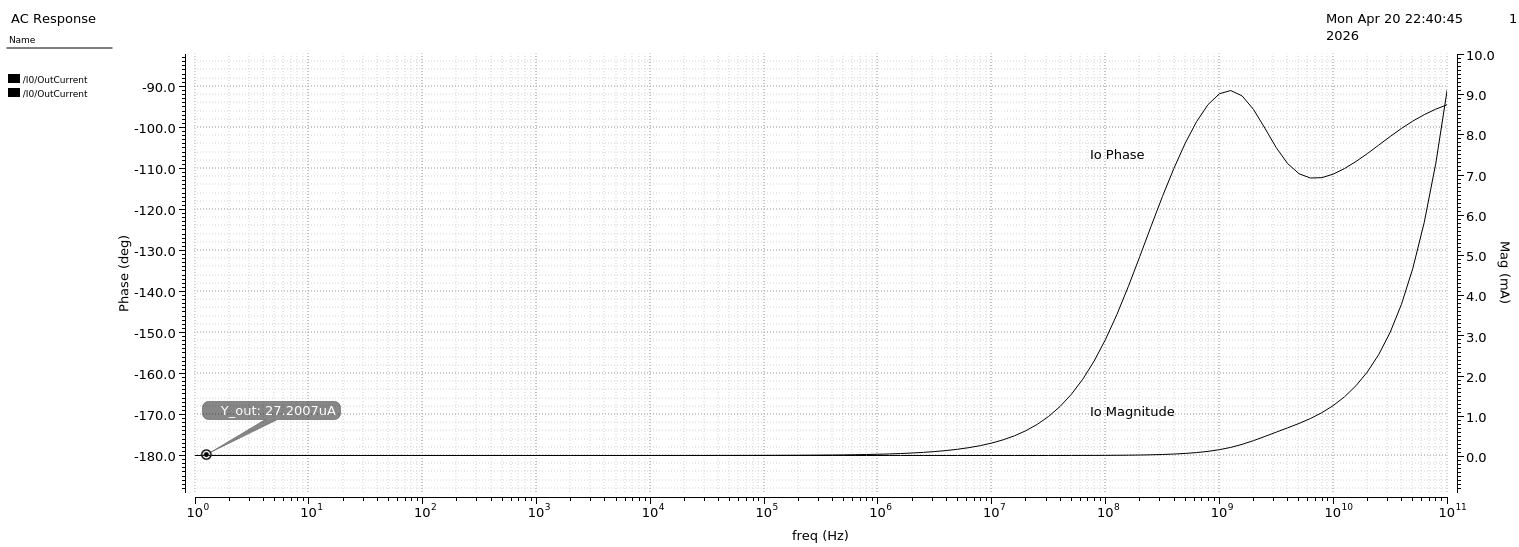
\includegraphics[width=0.8\linewidth]{chapters/miagesredone/Io_phase_mag.png}
    \caption{Magnitude and phase of the small signal output current}
\end{figure}

From the low-frequency value of the admittance magnitude:

\begin{equation*}
|Y_{out}(0)| = 27.2\,\mu\text{S}
\end{equation*}
the output resistance is then estimated as:

\begin{equation*}
R_o = \frac{1}{|Y_{out}(0)|} = 36.76\,\text{k}\Omega
\end{equation*}

\subsection{Output current error}
A DC sweep of the output voltage $V_{OUT}$ has been performed. First, the quantity $|V_{OUT} - V_{IN}|$ has been plotted as a function of $V_{OUT}$. Then, the output current error $|I_{OUT} - 5I_{REF}|$ has been plotted over the same sweep.

The operating point is identified as the value of $V_{OUT}$ for which the condition $|V_{OUT} - V_{IN}| = 0.4\,\text{V}$ is satisfied. By placing markers on the corresponding points of the two plots, the output current error is graphically extracted at the required condition.
% Missing \caption element inside
\begin{figure}[H]
    \centering
    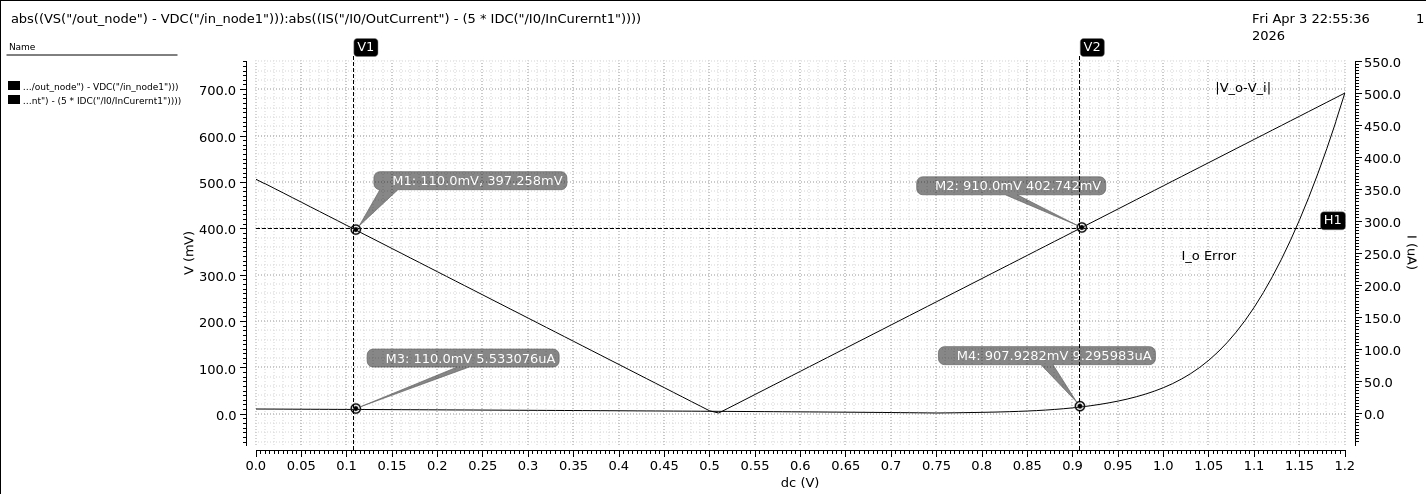
\includegraphics[width=1.00\linewidth]{imagesV2/part3_final.jpg}
    \caption{Output current error $|I_{OUT} - 5I_{REF}|$ and voltage deviation $|V_{OUT} - V_{IN}|$ vs $V_{OUT}$.}
    \label{fig:current_error}
\end{figure}
\subsubsection{Interpretation of the Current Error}
Although two operating points satisfy the required condition, only the right one on the graph(corresponding to the higher value of $V_{OUT}$) is physically meaningful. The first point occurs at low $V_{OUT}$, where the transistors are close to leaving the saturation region, thus violating the proper operating conditions of the current mirror.

Therefore, the current error is evaluated at the second intersection point, where the circuit operates correctly in saturation. The extracted value is:

\begin{equation*}
\Delta I_{OUT} \approx 9.3\,\mu\text{A}
\end{equation*}
In order to increase the output resistance of the cascode current mirror, the transistor dimensions have been scaled.
\subsection{Sizing approach for output resistance optimization}
Since the output resistance can be approximated as:
\begin{equation*}
R_o \approx g'_{m4} \cdot r_{o4} \cdot r_{o2}
\end{equation*}
it follows that, for constant current, the output resistance scales approximately as:
\begin{equation*}
R_o \propto L^2
\end{equation*}

For this reason, a first scaling factor $k = \sqrt{3}$ has been considered. This value is derived from the theoretical quadratic dependence of $R_o$ on the channel length and therefore represents only an ideal estimation.

The channel lengths of all transistors ($M_1$--$M_6$) have been increased by this factor. In order to preserve the aspect ratios and avoid modifying the bias currents, the widths have also been scaled accordingly for all transistors except $M_5$.

For transistor $M_5$, which acts as a biasing device, a rule-of-thumb has been adopted:
\begin{equation*}
W_5 = \frac{W_6}{3}
\end{equation*}

This choice allows proper biasing of the cascode branch. The operating point confirms that all transistors remain in saturation, including $M_5$.

\vspace{0.3cm}

From a theoretical point of view:
\begin{equation*}
R_o^{(th)} = 3 \cdot R_o = 3 \cdot 36.76\,\text{k}\Omega \approx 110\,\text{k}\Omega
\end{equation*}

However, simulation results show a different behaviour. From the AC analysis, the low-frequency output admittance is:
% Measunmet unit was A
\begin{equation*}
Y_{out}^{(sim)}(0) = 6.81\,\mu\text{S}
\end{equation*}
from which the output resistance is extracted as:
\begin{equation*}
R_o^{(sim)} = \frac{1}{Y_{out}^{(sim)}(0)} \approx 146.8\,\text{k}\Omega
\end{equation*}

This result highlights a deviation from the simplified model. However, the achieved design shows that both the systematic error and the mismatch of the output current are significantly reduced. This improvement comes at the cost of an increased occupied area (factor of $2.25$) coming with parasitic capacitances.

\begin{figure}[H]
    \centering
    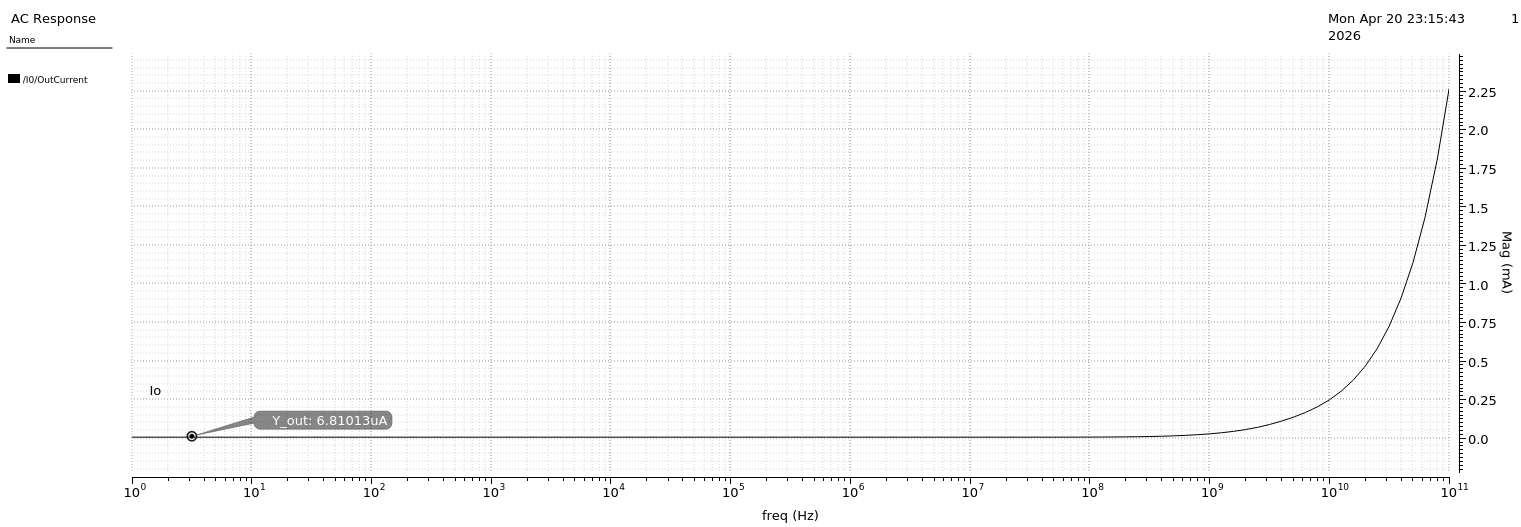
\includegraphics[width=1.0\linewidth]{chapters/miagesredone/Io_mag_cascode.png}
    \vspace{0.4cm}
    
    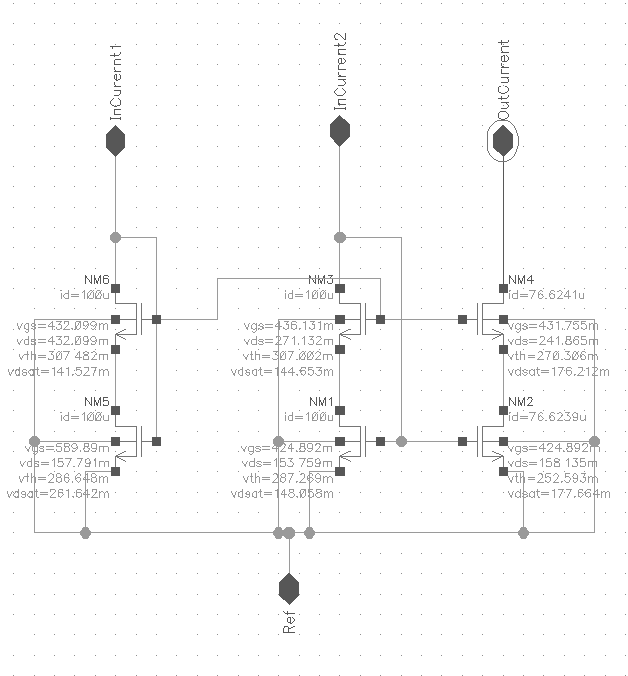
\includegraphics[width=0.6\linewidth]{chapters/miagesredone/schematics_cascode_op.png}
    
    \caption{Top: AC response used to extract the output admittance and compute $R_o^{(sim)}$. Bottom: operating point of the cascode mirror, showing that transistor $M_5$ is correctly biased in saturation.}
    \label{fig:cascode_rematch}
\end{figure}